% Options for packages loaded elsewhere
\PassOptionsToPackage{unicode}{hyperref}
\PassOptionsToPackage{hyphens}{url}
\PassOptionsToPackage{dvipsnames,svgnames,x11names}{xcolor}
%
\documentclass[
  letterpaper,
  DIV=11,
  numbers=noendperiod]{scrartcl}

\usepackage{amsmath,amssymb}
\usepackage{iftex}
\ifPDFTeX
  \usepackage[T1]{fontenc}
  \usepackage[utf8]{inputenc}
  \usepackage{textcomp} % provide euro and other symbols
\else % if luatex or xetex
  \usepackage{unicode-math}
  \defaultfontfeatures{Scale=MatchLowercase}
  \defaultfontfeatures[\rmfamily]{Ligatures=TeX,Scale=1}
\fi
\usepackage{lmodern}
\ifPDFTeX\else  
    % xetex/luatex font selection
\fi
% Use upquote if available, for straight quotes in verbatim environments
\IfFileExists{upquote.sty}{\usepackage{upquote}}{}
\IfFileExists{microtype.sty}{% use microtype if available
  \usepackage[]{microtype}
  \UseMicrotypeSet[protrusion]{basicmath} % disable protrusion for tt fonts
}{}
\makeatletter
\@ifundefined{KOMAClassName}{% if non-KOMA class
  \IfFileExists{parskip.sty}{%
    \usepackage{parskip}
  }{% else
    \setlength{\parindent}{0pt}
    \setlength{\parskip}{6pt plus 2pt minus 1pt}}
}{% if KOMA class
  \KOMAoptions{parskip=half}}
\makeatother
\usepackage{xcolor}
\setlength{\emergencystretch}{3em} % prevent overfull lines
\setcounter{secnumdepth}{-\maxdimen} % remove section numbering
% Make \paragraph and \subparagraph free-standing
\makeatletter
\ifx\paragraph\undefined\else
  \let\oldparagraph\paragraph
  \renewcommand{\paragraph}{
    \@ifstar
      \xxxParagraphStar
      \xxxParagraphNoStar
  }
  \newcommand{\xxxParagraphStar}[1]{\oldparagraph*{#1}\mbox{}}
  \newcommand{\xxxParagraphNoStar}[1]{\oldparagraph{#1}\mbox{}}
\fi
\ifx\subparagraph\undefined\else
  \let\oldsubparagraph\subparagraph
  \renewcommand{\subparagraph}{
    \@ifstar
      \xxxSubParagraphStar
      \xxxSubParagraphNoStar
  }
  \newcommand{\xxxSubParagraphStar}[1]{\oldsubparagraph*{#1}\mbox{}}
  \newcommand{\xxxSubParagraphNoStar}[1]{\oldsubparagraph{#1}\mbox{}}
\fi
\makeatother

\usepackage{color}
\usepackage{fancyvrb}
\newcommand{\VerbBar}{|}
\newcommand{\VERB}{\Verb[commandchars=\\\{\}]}
\DefineVerbatimEnvironment{Highlighting}{Verbatim}{commandchars=\\\{\}}
% Add ',fontsize=\small' for more characters per line
\usepackage{framed}
\definecolor{shadecolor}{RGB}{241,243,245}
\newenvironment{Shaded}{\begin{snugshade}}{\end{snugshade}}
\newcommand{\AlertTok}[1]{\textcolor[rgb]{0.68,0.00,0.00}{#1}}
\newcommand{\AnnotationTok}[1]{\textcolor[rgb]{0.37,0.37,0.37}{#1}}
\newcommand{\AttributeTok}[1]{\textcolor[rgb]{0.40,0.45,0.13}{#1}}
\newcommand{\BaseNTok}[1]{\textcolor[rgb]{0.68,0.00,0.00}{#1}}
\newcommand{\BuiltInTok}[1]{\textcolor[rgb]{0.00,0.23,0.31}{#1}}
\newcommand{\CharTok}[1]{\textcolor[rgb]{0.13,0.47,0.30}{#1}}
\newcommand{\CommentTok}[1]{\textcolor[rgb]{0.37,0.37,0.37}{#1}}
\newcommand{\CommentVarTok}[1]{\textcolor[rgb]{0.37,0.37,0.37}{\textit{#1}}}
\newcommand{\ConstantTok}[1]{\textcolor[rgb]{0.56,0.35,0.01}{#1}}
\newcommand{\ControlFlowTok}[1]{\textcolor[rgb]{0.00,0.23,0.31}{\textbf{#1}}}
\newcommand{\DataTypeTok}[1]{\textcolor[rgb]{0.68,0.00,0.00}{#1}}
\newcommand{\DecValTok}[1]{\textcolor[rgb]{0.68,0.00,0.00}{#1}}
\newcommand{\DocumentationTok}[1]{\textcolor[rgb]{0.37,0.37,0.37}{\textit{#1}}}
\newcommand{\ErrorTok}[1]{\textcolor[rgb]{0.68,0.00,0.00}{#1}}
\newcommand{\ExtensionTok}[1]{\textcolor[rgb]{0.00,0.23,0.31}{#1}}
\newcommand{\FloatTok}[1]{\textcolor[rgb]{0.68,0.00,0.00}{#1}}
\newcommand{\FunctionTok}[1]{\textcolor[rgb]{0.28,0.35,0.67}{#1}}
\newcommand{\ImportTok}[1]{\textcolor[rgb]{0.00,0.46,0.62}{#1}}
\newcommand{\InformationTok}[1]{\textcolor[rgb]{0.37,0.37,0.37}{#1}}
\newcommand{\KeywordTok}[1]{\textcolor[rgb]{0.00,0.23,0.31}{\textbf{#1}}}
\newcommand{\NormalTok}[1]{\textcolor[rgb]{0.00,0.23,0.31}{#1}}
\newcommand{\OperatorTok}[1]{\textcolor[rgb]{0.37,0.37,0.37}{#1}}
\newcommand{\OtherTok}[1]{\textcolor[rgb]{0.00,0.23,0.31}{#1}}
\newcommand{\PreprocessorTok}[1]{\textcolor[rgb]{0.68,0.00,0.00}{#1}}
\newcommand{\RegionMarkerTok}[1]{\textcolor[rgb]{0.00,0.23,0.31}{#1}}
\newcommand{\SpecialCharTok}[1]{\textcolor[rgb]{0.37,0.37,0.37}{#1}}
\newcommand{\SpecialStringTok}[1]{\textcolor[rgb]{0.13,0.47,0.30}{#1}}
\newcommand{\StringTok}[1]{\textcolor[rgb]{0.13,0.47,0.30}{#1}}
\newcommand{\VariableTok}[1]{\textcolor[rgb]{0.07,0.07,0.07}{#1}}
\newcommand{\VerbatimStringTok}[1]{\textcolor[rgb]{0.13,0.47,0.30}{#1}}
\newcommand{\WarningTok}[1]{\textcolor[rgb]{0.37,0.37,0.37}{\textit{#1}}}

\providecommand{\tightlist}{%
  \setlength{\itemsep}{0pt}\setlength{\parskip}{0pt}}\usepackage{longtable,booktabs,array}
\usepackage{calc} % for calculating minipage widths
% Correct order of tables after \paragraph or \subparagraph
\usepackage{etoolbox}
\makeatletter
\patchcmd\longtable{\par}{\if@noskipsec\mbox{}\fi\par}{}{}
\makeatother
% Allow footnotes in longtable head/foot
\IfFileExists{footnotehyper.sty}{\usepackage{footnotehyper}}{\usepackage{footnote}}
\makesavenoteenv{longtable}
\usepackage{graphicx}
\makeatletter
\newsavebox\pandoc@box
\newcommand*\pandocbounded[1]{% scales image to fit in text height/width
  \sbox\pandoc@box{#1}%
  \Gscale@div\@tempa{\textheight}{\dimexpr\ht\pandoc@box+\dp\pandoc@box\relax}%
  \Gscale@div\@tempb{\linewidth}{\wd\pandoc@box}%
  \ifdim\@tempb\p@<\@tempa\p@\let\@tempa\@tempb\fi% select the smaller of both
  \ifdim\@tempa\p@<\p@\scalebox{\@tempa}{\usebox\pandoc@box}%
  \else\usebox{\pandoc@box}%
  \fi%
}
% Set default figure placement to htbp
\def\fps@figure{htbp}
\makeatother

\usepackage{booktabs}
\usepackage{longtable}
\usepackage{array}
\usepackage{multirow}
\usepackage{wrapfig}
\usepackage{float}
\usepackage{colortbl}
\usepackage{pdflscape}
\usepackage{tabu}
\usepackage{threeparttable}
\usepackage{threeparttablex}
\usepackage[normalem]{ulem}
\usepackage{makecell}
\usepackage{xcolor}
\usepackage{caption}
\usepackage{anyfontsize}
\KOMAoption{captions}{tableheading}
\makeatletter
\@ifpackageloaded{caption}{}{\usepackage{caption}}
\AtBeginDocument{%
\ifdefined\contentsname
  \renewcommand*\contentsname{Table of contents}
\else
  \newcommand\contentsname{Table of contents}
\fi
\ifdefined\listfigurename
  \renewcommand*\listfigurename{List of Figures}
\else
  \newcommand\listfigurename{List of Figures}
\fi
\ifdefined\listtablename
  \renewcommand*\listtablename{List of Tables}
\else
  \newcommand\listtablename{List of Tables}
\fi
\ifdefined\figurename
  \renewcommand*\figurename{Figure}
\else
  \newcommand\figurename{Figure}
\fi
\ifdefined\tablename
  \renewcommand*\tablename{Table}
\else
  \newcommand\tablename{Table}
\fi
}
\@ifpackageloaded{float}{}{\usepackage{float}}
\floatstyle{ruled}
\@ifundefined{c@chapter}{\newfloat{codelisting}{h}{lop}}{\newfloat{codelisting}{h}{lop}[chapter]}
\floatname{codelisting}{Listing}
\newcommand*\listoflistings{\listof{codelisting}{List of Listings}}
\makeatother
\makeatletter
\makeatother
\makeatletter
\@ifpackageloaded{caption}{}{\usepackage{caption}}
\@ifpackageloaded{subcaption}{}{\usepackage{subcaption}}
\makeatother

\usepackage{bookmark}

\IfFileExists{xurl.sty}{\usepackage{xurl}}{} % add URL line breaks if available
\urlstyle{same} % disable monospaced font for URLs
\hypersetup{
  pdftitle={Modele\_IV},
  pdfauthor={YAMEOGO Saïdou},
  colorlinks=true,
  linkcolor={blue},
  filecolor={Maroon},
  citecolor={Blue},
  urlcolor={Blue},
  pdfcreator={LaTeX via pandoc}}


\title{Modele\_IV}
\author{YAMEOGO Saïdou}
\date{}

\begin{document}
\maketitle


\subsection{Quarto}\label{quarto}

You can add options to executable code like this

\begin{verbatim}
[1] 4
\end{verbatim}

\section{formulation de la
modelisation}\label{formulation-de-la-modelisation}

Nous voulons estimer l'effet de l'éducation sur les salaires en
utilisant un appareil différent - la proximité géographique des
collèges. Ces données proviennent de l'étude de David Card de 1995 où il
a fait la même chose, et elle est disponible dans la bibliothèque
«wooldridge» comme card.

\subsubsection{Description des
variables}\label{description-des-variables}

lwage : Salaire annuel (formulaire journalier) educ : Années d'éducation
nearc4 : Vivre à proximité de l'université (1 dollar) ou loin de
l'université (0 dollar) smsa : Vivant dans la zone métropolitaine (no 1)
ou non (-0) exper : Années d'expérience expersq : Années d'expérience
(terme de marché) black : Noir (no 1), pas noir (-0) south : Vivant dans
le sud (no 1) ou non (-0)

Les variables smsa66, exper, expersq , black, south66 sont des variables
de contrôle (C'est - à- dire que le salaire expliqué en plus de
l'éducation par ces variables). Par contre dans la réalité nous
constatons que l'éducation même est influencée par d'autres variables
comme l'approximité de l'université. Nous supçonnons donc la variable
éducation d'être endogène.

\subsection{Les packages}\label{les-packages}

\begin{Shaded}
\begin{Highlighting}[]
\FunctionTok{library}\NormalTok{(tidyverse)  }\CommentTok{\# ggplot(), mutate(), and friends}
\end{Highlighting}
\end{Shaded}

\begin{verbatim}
Warning: le package 'tidyverse' a été compilé avec la version R 4.4.3
\end{verbatim}

\begin{verbatim}
Warning: le package 'ggplot2' a été compilé avec la version R 4.4.3
\end{verbatim}

\begin{verbatim}
Warning: le package 'readr' a été compilé avec la version R 4.4.3
\end{verbatim}

\begin{verbatim}
Warning: le package 'purrr' a été compilé avec la version R 4.4.3
\end{verbatim}

\begin{verbatim}
Warning: le package 'dplyr' a été compilé avec la version R 4.4.3
\end{verbatim}

\begin{verbatim}
Warning: le package 'forcats' a été compilé avec la version R 4.4.3
\end{verbatim}

\begin{verbatim}
Warning: le package 'lubridate' a été compilé avec la version R 4.4.3
\end{verbatim}

\begin{verbatim}
-- Attaching core tidyverse packages ------------------------ tidyverse 2.0.0 --
v dplyr     1.1.4     v readr     2.1.5
v forcats   1.0.0     v stringr   1.5.1
v ggplot2   3.5.2     v tibble    3.2.1
v lubridate 1.9.4     v tidyr     1.3.1
v purrr     1.0.4     
-- Conflicts ------------------------------------------ tidyverse_conflicts() --
x dplyr::filter() masks stats::filter()
x dplyr::lag()    masks stats::lag()
i Use the conflicted package (<http://conflicted.r-lib.org/>) to force all conflicts to become errors
\end{verbatim}

\begin{Shaded}
\begin{Highlighting}[]
\FunctionTok{library}\NormalTok{(broom)  }\CommentTok{\# Convert models to data frames}
\end{Highlighting}
\end{Shaded}

\begin{verbatim}
Warning: le package 'broom' a été compilé avec la version R 4.4.3
\end{verbatim}

\begin{Shaded}
\begin{Highlighting}[]
\FunctionTok{library}\NormalTok{(modelsummary)  }\CommentTok{\# Create side{-}by{-}side regression tables}
\end{Highlighting}
\end{Shaded}

\begin{verbatim}
Warning: le package 'modelsummary' a été compilé avec la version R 4.4.3
\end{verbatim}

\begin{Shaded}
\begin{Highlighting}[]
\FunctionTok{library}\NormalTok{(kableExtra)  }\CommentTok{\# Add fancier formatting to tables}
\end{Highlighting}
\end{Shaded}

\begin{verbatim}
Warning: le package 'kableExtra' a été compilé avec la version R 4.4.3
\end{verbatim}

\begin{verbatim}

Attachement du package : 'kableExtra'

L'objet suivant est masqué depuis 'package:dplyr':

    group_rows
\end{verbatim}

\begin{Shaded}
\begin{Highlighting}[]
\FunctionTok{library}\NormalTok{(estimatr)  }\CommentTok{\# Run 2SLS models in one step with iv\_robust()}
\end{Highlighting}
\end{Shaded}

\begin{verbatim}
Warning: le package 'estimatr' a été compilé avec la version R 4.4.3
\end{verbatim}

\begin{Shaded}
\begin{Highlighting}[]
\FunctionTok{library}\NormalTok{(dplyr)}
\FunctionTok{library}\NormalTok{(AER) }\CommentTok{\# Pour les models instrumentaux (iv)}
\end{Highlighting}
\end{Shaded}

\begin{verbatim}
Warning: le package 'AER' a été compilé avec la version R 4.4.3
\end{verbatim}

\begin{verbatim}
Le chargement a nécessité le package : car
\end{verbatim}

\begin{verbatim}
Warning: le package 'car' a été compilé avec la version R 4.4.3
\end{verbatim}

\begin{verbatim}
Le chargement a nécessité le package : carData
\end{verbatim}

\begin{verbatim}
Warning: le package 'carData' a été compilé avec la version R 4.4.3
\end{verbatim}

\begin{verbatim}

Attachement du package : 'car'

L'objet suivant est masqué depuis 'package:dplyr':

    recode

L'objet suivant est masqué depuis 'package:purrr':

    some

Le chargement a nécessité le package : lmtest
\end{verbatim}

\begin{verbatim}
Warning: le package 'lmtest' a été compilé avec la version R 4.4.3
\end{verbatim}

\begin{verbatim}
Le chargement a nécessité le package : zoo
\end{verbatim}

\begin{verbatim}
Warning: le package 'zoo' a été compilé avec la version R 4.4.3
\end{verbatim}

\begin{verbatim}

Attachement du package : 'zoo'

Les objets suivants sont masqués depuis 'package:base':

    as.Date, as.Date.numeric

Le chargement a nécessité le package : sandwich
\end{verbatim}

\begin{verbatim}
Warning: le package 'sandwich' a été compilé avec la version R 4.4.3
\end{verbatim}

\begin{verbatim}
Le chargement a nécessité le package : survival
\end{verbatim}

\begin{verbatim}
Warning: le package 'survival' a été compilé avec la version R 4.4.3
\end{verbatim}

\begin{Shaded}
\begin{Highlighting}[]
\FunctionTok{library}\NormalTok{(plm) }\CommentTok{\#Pour le test de hausman}
\end{Highlighting}
\end{Shaded}

\begin{verbatim}
Warning: le package 'plm' a été compilé avec la version R 4.4.3
\end{verbatim}

\begin{verbatim}

Attachement du package : 'plm'

Les objets suivants sont masqués depuis 'package:dplyr':

    between, lag, lead
\end{verbatim}

\begin{Shaded}
\begin{Highlighting}[]
\FunctionTok{library}\NormalTok{(ggplot2)}
\end{Highlighting}
\end{Shaded}

\section{Importation de la base de
données}\label{importation-de-la-base-de-donnuxe9es}

\begin{Shaded}
\begin{Highlighting}[]
\NormalTok{base }\OtherTok{\textless{}{-}} \FunctionTok{read.csv}\NormalTok{(}\StringTok{"base\_educ.csv"}\NormalTok{, }\AttributeTok{sep =} \StringTok{","}\NormalTok{) }\SpecialCharTok{\%\textgreater{}\%}
  \FunctionTok{select}\NormalTok{(}\FunctionTok{all\_of}\NormalTok{(}\FunctionTok{c}\NormalTok{(}\StringTok{"lwage"}\NormalTok{, }\StringTok{"educ"}\NormalTok{, }\StringTok{"nearc4"}\NormalTok{, }\StringTok{"exper"}\NormalTok{, }\StringTok{"expersq"}\NormalTok{, }\StringTok{"black"}\NormalTok{, }\StringTok{"south66"}\NormalTok{))) }\SpecialCharTok{\%\textgreater{}\%}
  \FunctionTok{rename}\NormalTok{(}
    \AttributeTok{salaire =}\NormalTok{ lwage,}
    \AttributeTok{education =}\NormalTok{ educ,}
    \AttributeTok{proximite =}\NormalTok{ nearc4,}
    \CommentTok{\#zone = smsa66,}
    \AttributeTok{experience =}\NormalTok{ exper,}
    \AttributeTok{exper\_marche =}\NormalTok{ expersq,}
    \AttributeTok{race\_noir =}\NormalTok{ black,}
    \AttributeTok{sud =}\NormalTok{ south66}
\NormalTok{  ) }\SpecialCharTok{\%\textgreater{}\%}
  \FunctionTok{na.omit}\NormalTok{()}
\end{Highlighting}
\end{Shaded}

\section{Vérification de l'endogénéité de la variable explicative
(education)}\label{vuxe9rification-de-lendoguxe9nuxe9ituxe9-de-la-variable-explicative-education}

Comme formuler plus haut nous supçonnons la variable education d'être
endogène, pour cela nous allons faire le test de Hausman pour verifier
cela en considerant l'approximité comme la variable instrumentale.

\subsection{Etape 1: Le modèle naïf : c'est le modèle estimé avec
MCO}\label{etape-1-le-moduxe8le-nauxeff-cest-le-moduxe8le-estimuxe9-avec-mco}

\subsubsection{L'équation du modèle naïf (estimé par MCO) s'écrit
:}\label{luxe9quation-du-moduxe8le-nauxeff-estimuxe9-par-mco-suxe9crit}

\[
\texttt{salaire} = \beta_0 + \beta_1 \cdot \texttt{education} + \beta_2 \cdot \texttt{sud} + \beta_3 \cdot \texttt{race_noir} + \beta_4 \cdot \texttt{exper_marche} + \beta_5 \cdot \texttt{experience}+ u_i
\]

\begin{Shaded}
\begin{Highlighting}[]
\NormalTok{model\_naif }\OtherTok{\textless{}{-}} \FunctionTok{lm}\NormalTok{(salaire }\SpecialCharTok{\textasciitilde{}}\NormalTok{ education }\SpecialCharTok{+}\NormalTok{ sud }\SpecialCharTok{+}\NormalTok{ race\_noir }\SpecialCharTok{+}\NormalTok{ exper\_marche }\SpecialCharTok{+}\NormalTok{ experience , }\AttributeTok{data =}\NormalTok{ base)}
\FunctionTok{summary}\NormalTok{(model\_naif)}
\end{Highlighting}
\end{Shaded}

\begin{verbatim}

Call:
lm(formula = salaire ~ education + sud + race_noir + exper_marche + 
    experience, data = base)

Residuals:
    Min      1Q  Median      3Q     Max 
-1.7106 -0.2403  0.0198  0.2565  1.3777 

Coefficients:
               Estimate Std. Error t value Pr(>|t|)    
(Intercept)   4.7758870  0.0690054  69.210  < 2e-16 ***
education     0.0786805  0.0035693  22.044  < 2e-16 ***
sud          -0.1224405  0.0158290  -7.735 1.40e-14 ***
race_noir    -0.1755865  0.0186444  -9.418  < 2e-16 ***
exper_marche -0.0024044  0.0003251  -7.395 1.82e-13 ***
experience    0.0862585  0.0068027  12.680  < 2e-16 ***
---
Signif. codes:  0 '***' 0.001 '**' 0.01 '*' 0.05 '.' 0.1 ' ' 1

Residual standard error: 0.3831 on 3004 degrees of freedom
Multiple R-squared:  0.2559,    Adjusted R-squared:  0.2546 
F-statistic: 206.6 on 5 and 3004 DF,  p-value: < 2.2e-16
\end{verbatim}

\subsection{Etape 2 : Le modèle instrumental (MI) (avec proximite comme
instrument)}\label{etape-2-le-moduxe8le-instrumental-mi-avec-proximite-comme-instrument}

\begin{Shaded}
\begin{Highlighting}[]
\NormalTok{iv\_model }\OtherTok{\textless{}{-}}\NormalTok{ AER}\SpecialCharTok{::}\FunctionTok{ivreg}\NormalTok{(salaire }\SpecialCharTok{\textasciitilde{}}\NormalTok{ education }\SpecialCharTok{+}\NormalTok{ sud }\SpecialCharTok{+}\NormalTok{race\_noir }\SpecialCharTok{+}\NormalTok{ exper\_marche }\SpecialCharTok{+}\NormalTok{ experience }\SpecialCharTok{|}
\NormalTok{                            proximite }\SpecialCharTok{+}\NormalTok{ sud }\SpecialCharTok{+}\NormalTok{ race\_noir }\SpecialCharTok{+}\NormalTok{ exper\_marche }\SpecialCharTok{+}\NormalTok{ experience ,}
                  \AttributeTok{data =}\NormalTok{ base)}


\CommentTok{\#summary(iv\_model)}
\end{Highlighting}
\end{Shaded}

\subsection{Etape 3 : Test de Hauman}\label{etape-3-test-de-hauman}

H\_0: Pas d'endogénéité. Les estimateurs MCO et 2SLS sont proches.
L'estimateur MCO est convergent. H\_1 : Présence d'endogénéité. Les
estimateurs MCO et 2SLS sont significativement différents. L'estimateur
MCO est biaisé et inconsistent.

La statistique est donnée par : \$\$

\begin{verbatim}
H = (\hat{\beta}_{\text{2SLS}} - \hat{\beta}_{\text{MCO}})' 
\left[
\text{Var}(\hat{\beta}_{\text{2SLS}}) - \text{Var}(\hat{\beta}_{\text{MCO}})
\right]^{-1}
(\hat{\beta}_{\text{2SLS}} - \hat{\beta}_{\text{MCO}})
\end{verbatim}

Décision

Si la statistique \(H\) est faible (valeur-p \textgreater{} 5\%) : On ne
rejette pas \(H_0\). Donc pas d'endogénéité et le modèle de MCO est
acceptable. Si la statistique \(H\) est

élevée\} (valeur-p \textless{} 5\%) : On rejette \(H_0\). Présence
d'endogénéité. Préférer l'estimateur 2SLS.

Le test

\begin{Shaded}
\begin{Highlighting}[]
\FunctionTok{summary}\NormalTok{(iv\_model, }\AttributeTok{diagnostics =} \ConstantTok{TRUE}\NormalTok{)}
\end{Highlighting}
\end{Shaded}

\begin{verbatim}

Call:
AER::ivreg(formula = salaire ~ education + sud + race_noir + 
    exper_marche + experience | proximite + sud + race_noir + 
    exper_marche + experience, data = base)

Residuals:
     Min       1Q   Median       3Q      Max 
-2.30716 -0.31527  0.01102  0.32674  1.84069 

Coefficients:
               Estimate Std. Error t value Pr(>|t|)    
(Intercept)   2.0593143  0.7765684   2.652  0.00805 ** 
education     0.2359817  0.0449075   5.255 1.59e-07 ***
sud          -0.0445780  0.0300256  -1.485  0.13774    
race_noir    -0.0325622  0.0471407  -0.691  0.48978    
exper_marche -0.0024579  0.0004175  -5.887 4.36e-09 ***
experience    0.1505826  0.0202464   7.438 1.33e-13 ***

Diagnostic tests:
                  df1  df2 statistic  p-value    
Weak instruments    1 3004     31.57 2.09e-08 ***
Wu-Hausman          1 3003     20.55 6.04e-06 ***
Sargan              0   NA        NA       NA    
---
Signif. codes:  0 '***' 0.001 '**' 0.01 '*' 0.05 '.' 0.1 ' ' 1

Residual standard error: 0.4916 on 3004 degrees of freedom
Multiple R-Squared: -0.2252,    Adjusted R-squared: -0.2273 
Wald test: 71.98 on 5 and 3004 DF,  p-value: < 2.2e-16 
\end{verbatim}

La p-value du test de Hausman est 6.04e-06 (largement inferieure à 5\%).
Donc on rejete HO et il y a présence d'endogénéité. Nous utiliserons
dans ce cas le modèle de régression linéaire à variable instrumentale.

\section{Les conditions de validité de l'instrument
(proximité)}\label{les-conditions-de-validituxe9-de-linstrument-proximituxe9}

\subsection{Vérifiez la validité de
l'instrument}\label{vuxe9rifiez-la-validituxe9-de-linstrument}

Pour qu'un instrument soit valable, il doit répondre à trois critères:

Pertinence: l'instrument est corrélé à la variable de politique

Exclusion : L'instrument n'est corrélé avec le résultat que par le biais
de la variable de la politique

Exogénité : L'instrument n'est pas corrélé avec quoi que ce soit d'autre
dans le modèle (c'est-à-dire les variables omises)

\#\#1. Pertinence (condition d'inclusion)

\begin{Shaded}
\begin{Highlighting}[]
\NormalTok{check\_pertinence}\OtherTok{\textless{}{-}} \FunctionTok{lm}\NormalTok{(education }\SpecialCharTok{\textasciitilde{}}\NormalTok{ proximite }\SpecialCharTok{+}\NormalTok{ sud  }\SpecialCharTok{+}\NormalTok{ exper\_marche }\SpecialCharTok{+}\NormalTok{ experience }\SpecialCharTok{+}\NormalTok{ race\_noir,}
                      \AttributeTok{data =}\NormalTok{ base)}
\FunctionTok{tidy}\NormalTok{(check\_pertinence)}
\end{Highlighting}
\end{Shaded}

\begin{verbatim}
# A tibble: 6 x 5
  term          estimate std.error statistic  p.value
  <chr>            <dbl>     <dbl>     <dbl>    <dbl>
1 (Intercept)  16.9        0.170      99.6   0       
2 proximite     0.444      0.0790      5.62  2.09e- 8
3 sud          -0.382      0.0825     -4.63  3.76e- 6
4 exper_marche  0.000433   0.00165     0.262 7.94e- 1
5 experience   -0.409      0.0338    -12.1   5.85e-33
6 race_noir    -0.931      0.0934     -9.97  4.81e-23
\end{verbatim}

\begin{Shaded}
\begin{Highlighting}[]
\FunctionTok{glance}\NormalTok{(check\_pertinence)}
\end{Highlighting}
\end{Shaded}

\begin{verbatim}
# A tibble: 1 x 12
  r.squared adj.r.squared sigma statistic p.value    df logLik    AIC    BIC
      <dbl>         <dbl> <dbl>     <dbl>   <dbl> <dbl>  <dbl>  <dbl>  <dbl>
1     0.471         0.470  1.95      535.       0     5 -6276. 12565. 12607.
# i 3 more variables: deviance <dbl>, df.residual <int>, nobs <int>
\end{verbatim}

Decision La statistique F est nettement supérieure à 20 (c'est
535,2301),D'après la règle empirique de Stock-Yogo, l'intrument est
fort. Il existe une relation significative entre l'instrument et
l'éducation (p-value =2.094877e-08) . L'instrument est donc pertinent

\subsection{2. exclusion}\label{exclusion}

Exclusion

Pour vérifier l'exclusion, nous devons voir s'il y a une relation entre
l'éducation des pères et les salaires qui ne se produit que grâce à
l'éducation. Si nous complotons, nous verrons une relation :

\begin{Shaded}
\begin{Highlighting}[]
\CommentTok{\# install.packages("ggdag")}
\FunctionTok{library}\NormalTok{(ggdag)}
\end{Highlighting}
\end{Shaded}

\begin{verbatim}
Warning: le package 'ggdag' a été compilé avec la version R 4.4.3
\end{verbatim}

\begin{verbatim}

Attachement du package : 'ggdag'
\end{verbatim}

\begin{verbatim}
L'objet suivant est masqué depuis 'package:stats':

    filter
\end{verbatim}

\begin{Shaded}
\begin{Highlighting}[]
\NormalTok{dag }\OtherTok{\textless{}{-}} \FunctionTok{dagify}\NormalTok{(}
\NormalTok{  salaire }\SpecialCharTok{\textasciitilde{}}\NormalTok{ education }\SpecialCharTok{+}\NormalTok{ experience }\SpecialCharTok{+}\NormalTok{ race\_noir }\SpecialCharTok{+}\NormalTok{ sud ,}
\NormalTok{  education }\SpecialCharTok{\textasciitilde{}}\NormalTok{ proximite }\SpecialCharTok{+}\NormalTok{ experience }\SpecialCharTok{+}\NormalTok{ race\_noir }\SpecialCharTok{+}\NormalTok{ sud ,}
  \AttributeTok{exposure =} \StringTok{"education"}\NormalTok{,}
  \AttributeTok{outcome =} \StringTok{"salaire"}
\NormalTok{)}

\FunctionTok{ggdag}\NormalTok{(dag, }\AttributeTok{layout =} \StringTok{"circle"}\NormalTok{) }\SpecialCharTok{+}
  \FunctionTok{theme\_dag}\NormalTok{()}
\end{Highlighting}
\end{Shaded}

\pandocbounded{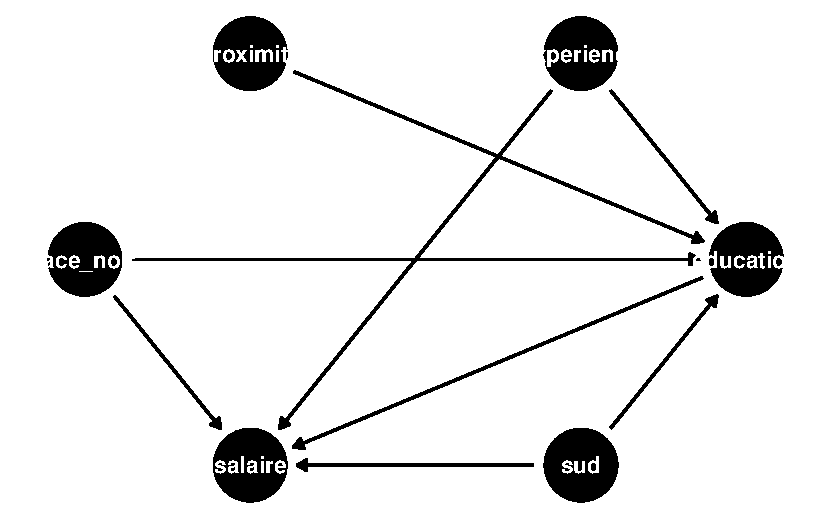
\includegraphics[keepaspectratio]{projet_VI_files/figure-pdf/unnamed-chunk-8-1.pdf}}

Maintenant que l'instrument est valide, nous allons passer à
l'estimation des parametres du modèle par la Double Moindre Carrée.

\#Estimation des paramètres par le DMCO

\subsection{Etape 1 :Régression
auxiliaire}\label{etape-1-ruxe9gression-auxiliaire}

\[
\texttt{education} = \gamma_0 + \gamma_1 \cdot \texttt{proximite} + \gamma_2 \cdot \texttt{sud} + \gamma_3 \cdot \texttt{race_noir} + \gamma_4 \cdot \texttt{exper_marche} + \gamma_5 \cdot \texttt{experience} + \varepsilon_i
\]

\begin{Shaded}
\begin{Highlighting}[]
\NormalTok{model\_aux }\OtherTok{\textless{}{-}} \FunctionTok{lm}\NormalTok{(education }\SpecialCharTok{\textasciitilde{}}\NormalTok{ proximite }\SpecialCharTok{+}\NormalTok{ sud }\SpecialCharTok{+}\NormalTok{ race\_noir }\SpecialCharTok{+}\NormalTok{ exper\_marche }\SpecialCharTok{+}\NormalTok{ experience, }\AttributeTok{data =}\NormalTok{ base)}
\FunctionTok{tidy}\NormalTok{(model\_aux)}
\end{Highlighting}
\end{Shaded}

\begin{verbatim}
# A tibble: 6 x 5
  term          estimate std.error statistic  p.value
  <chr>            <dbl>     <dbl>     <dbl>    <dbl>
1 (Intercept)  16.9        0.170      99.6   0       
2 proximite     0.444      0.0790      5.62  2.09e- 8
3 sud          -0.382      0.0825     -4.63  3.76e- 6
4 race_noir    -0.931      0.0934     -9.97  4.81e-23
5 exper_marche  0.000433   0.00165     0.262 7.94e- 1
6 experience   -0.409      0.0338    -12.1   5.85e-33
\end{verbatim}

Nous pouvons alors extraire l'éducation prévue et l'ajouter à notre
principal ensemble de données, rebaptisant le .fitted variable à quelque
chose de plus utile en cours de route:

\begin{Shaded}
\begin{Highlighting}[]
\NormalTok{base\_avec\_predit }\OtherTok{\textless{}{-}} \FunctionTok{augment\_columns}\NormalTok{(model\_aux, base) }\SpecialCharTok{|\textgreater{}}
  \FunctionTok{rename}\NormalTok{(}\AttributeTok{education\_estim =}\NormalTok{ .fitted)}
\end{Highlighting}
\end{Shaded}

\begin{Shaded}
\begin{Highlighting}[]
\NormalTok{base\_avec\_predit}
\end{Highlighting}
\end{Shaded}

\begin{verbatim}
# A tibble: 3,010 x 14
   salaire education proximite experience exper_marche race_noir   sud
     <dbl>     <int>     <int>      <int>        <int>     <int> <int>
 1    6.31         7         0         16          256         1     0
 2    6.18        12         0          9           81         0     0
 3    6.58        12         0         16          256         0     0
 4    5.52        11         1         10          100         0     0
 5    6.59        12         1         16          256         0     0
 6    6.21        12         1          8           64         0     0
 7    6.34        18         1          9           81         0     0
 8    6.41        14         1          9           81         0     0
 9    6.05        12         1         10          100         0     0
10    6.24        12         1         11          121         0     0
# i 3,000 more rows
# i 7 more variables: education_estim <dbl>, .se.fit <dbl>, .resid <dbl>,
#   .hat <dbl>, .sigma <dbl>, .cooksd <dbl>, .std.resid <dbl>
\end{verbatim}

\subsection{Etape 2 : Estimation avec l'education
estimée}\label{etape-2-estimation-avec-leducation-estimuxe9e}

Enfin, nous pouvons utiliser l'éducation prévue pour estimer l'effet
exogène de l'éducation sur les salaires:

\begin{Shaded}
\begin{Highlighting}[]
\NormalTok{model2 }\OtherTok{\textless{}{-}} \FunctionTok{lm}\NormalTok{(salaire }\SpecialCharTok{\textasciitilde{}}\NormalTok{ education\_estim }\SpecialCharTok{+}\NormalTok{sud }\SpecialCharTok{+}\NormalTok{ race\_noir }\SpecialCharTok{+}\NormalTok{ exper\_marche }\SpecialCharTok{+}\NormalTok{ experience,}
                   \AttributeTok{data =}\NormalTok{ base\_avec\_predit)}
\FunctionTok{tidy}\NormalTok{(model2)}
\end{Highlighting}
\end{Shaded}

\begin{verbatim}
# A tibble: 6 x 5
  term            estimate std.error statistic  p.value
  <chr>              <dbl>     <dbl>     <dbl>    <dbl>
1 (Intercept)      2.06     0.648        3.18  1.50e- 3
2 education_estim  0.236    0.0375       6.30  3.48e-10
3 sud             -0.0446   0.0251      -1.78  7.53e- 2
4 race_noir       -0.0326   0.0393      -0.828 4.08e- 1
5 exper_marche    -0.00246  0.000348    -7.06  2.13e-12
6 experience       0.151    0.0169       8.91  8.46e-19
\end{verbatim}

\section{Reprenons avec l'estimation en une seule
étape}\label{reprenons-avec-lestimation-en-une-seule-uxe9tape}

\begin{Shaded}
\begin{Highlighting}[]
\NormalTok{model\_2sls }\OtherTok{\textless{}{-}} \FunctionTok{iv\_robust}\NormalTok{(salaire }\SpecialCharTok{\textasciitilde{}}\NormalTok{ education }\SpecialCharTok{+}\NormalTok{ sud  }\SpecialCharTok{+}\NormalTok{ exper\_marche }\SpecialCharTok{+}\NormalTok{ experience }\SpecialCharTok{+}\NormalTok{ race\_noir  }\SpecialCharTok{|}
\NormalTok{                            proximite }\SpecialCharTok{+}\NormalTok{ sud }\SpecialCharTok{+}\NormalTok{ race\_noir }\SpecialCharTok{+}\NormalTok{ exper\_marche }\SpecialCharTok{+}\NormalTok{ experience ,}
                        \AttributeTok{data =}\NormalTok{ base, }\AttributeTok{diagnostics =} \ConstantTok{TRUE}\NormalTok{)}
\FunctionTok{tidy}\NormalTok{(model\_2sls)}
\end{Highlighting}
\end{Shaded}

\begin{verbatim}
          term     estimate    std.error  statistic      p.value     conf.low
1  (Intercept)  2.059314288 0.7692793913  2.6769394 7.470198e-03  0.550946643
2    education  0.235981673 0.0445477592  5.2972737 1.260309e-07  0.148634476
3          sud -0.044578003 0.0299768663 -1.4870801 1.370986e-01 -0.103355263
4 exper_marche -0.002457891 0.0004478504 -5.4881967 4.398435e-08 -0.003336016
5   experience  0.150582586 0.0201192804  7.4844917 9.381642e-14  0.111133627
6    race_noir -0.032562248 0.0456081279 -0.7139571 4.753092e-01 -0.121988568
     conf.high   df outcome
1  3.567681933 3004 salaire
2  0.323328871 3004 salaire
3  0.014199258 3004 salaire
4 -0.001579767 3004 salaire
5  0.190031546 3004 salaire
6  0.056864071 3004 salaire
\end{verbatim}

\subsection{Comparaison des resultats}\label{comparaison-des-resultats}

\begin{Shaded}
\begin{Highlighting}[]
\FunctionTok{modelsummary}\NormalTok{(}
  \FunctionTok{list}\NormalTok{(}\StringTok{"OLS"} \OtherTok{=}\NormalTok{ model\_naif, }\StringTok{"2SLS (automatic)"} \OtherTok{=}\NormalTok{ model\_2sls),}
  \AttributeTok{gof\_omit =} \StringTok{"IC|Log|Adj|p}\SpecialCharTok{\textbackslash{}\textbackslash{}}\StringTok{.value|statistic|se\_type"}\NormalTok{,}
  \AttributeTok{stars =} \ConstantTok{TRUE}\NormalTok{,}
  \AttributeTok{output =} \StringTok{"gt"}
\NormalTok{) }\SpecialCharTok{|\textgreater{}}
\NormalTok{  gt}\SpecialCharTok{::}\FunctionTok{tab\_style}\NormalTok{(}
    \AttributeTok{style =}\NormalTok{ gt}\SpecialCharTok{::}\FunctionTok{cell\_fill}\NormalTok{(}\AttributeTok{color =} \StringTok{"\#FF3"}\NormalTok{),}
    \AttributeTok{locations =}\NormalTok{ gt}\SpecialCharTok{::}\FunctionTok{cells\_body}\NormalTok{(}\AttributeTok{rows =} \FunctionTok{c}\NormalTok{(}\DecValTok{3}\NormalTok{, }\DecValTok{5}\NormalTok{))}
\NormalTok{  )}
\end{Highlighting}
\end{Shaded}

\begin{table}
\fontsize{12.0pt}{14.4pt}\selectfont
\begin{tabular*}{\linewidth}{@{\extracolsep{\fill}}lcc}
\toprule
  & OLS & 2SLS (automatic) \\ 
\midrule\addlinespace[2.5pt]
(Intercept) & 4.776*** & 2.059** \\ 
 & (0.069) & (0.769) \\ 
{\cellcolor[HTML]{FFFF33}{education}} & {\cellcolor[HTML]{FFFF33}{0.079***}} & {\cellcolor[HTML]{FFFF33}{0.236***}} \\ 
 & (0.004) & (0.045) \\ 
{\cellcolor[HTML]{FFFF33}{sud}} & {\cellcolor[HTML]{FFFF33}{-0.122***}} & {\cellcolor[HTML]{FFFF33}{-0.045}} \\ 
 & (0.016) & (0.030) \\ 
race\_noir & -0.176*** & -0.033 \\ 
 & (0.019) & (0.046) \\ 
exper\_marche & -0.002*** & -0.002*** \\ 
 & (0.000) & (0.000) \\ 
experience & 0.086*** & 0.151*** \\ 
{} & {(0.007)} & {(0.020)} \\ 
Num.Obs. & 3010 & 3010 \\ 
R2 & 0.256 & -0.225 \\ 
F & 206.605 &  \\ 
RMSE & 0.38 & 0.49 \\ 
\bottomrule
\end{tabular*}
\begin{minipage}{\linewidth}
+ p < 0.1, * p < 0.05, ** p < 0.01, *** p < 0.001\\
\end{minipage}
\end{table}

\begin{Shaded}
\begin{Highlighting}[]
\CommentTok{\# Suppose que tu as un data.frame \textquotesingle{}base\textquotesingle{} avec salaire et education}
\FunctionTok{ggplot}\NormalTok{(base, }\FunctionTok{aes}\NormalTok{(}\AttributeTok{x =}\NormalTok{ education, }\AttributeTok{y =}\NormalTok{ salaire)) }\SpecialCharTok{+}
  \FunctionTok{geom\_point}\NormalTok{(}\AttributeTok{alpha =} \FloatTok{0.3}\NormalTok{) }\SpecialCharTok{+}
  \FunctionTok{geom\_smooth}\NormalTok{(}\AttributeTok{method =} \StringTok{"lm"}\NormalTok{, }\AttributeTok{se =} \ConstantTok{FALSE}\NormalTok{, }\AttributeTok{color =} \StringTok{"blue"}\NormalTok{, }\AttributeTok{linetype =} \StringTok{"dashed"}\NormalTok{) }\SpecialCharTok{+}  \CommentTok{\# OLS}
  \FunctionTok{geom\_abline}\NormalTok{(}\AttributeTok{intercept =} \FloatTok{2.06}\NormalTok{, }\AttributeTok{slope =} \FloatTok{0.2359}\NormalTok{, }\AttributeTok{color =} \StringTok{"red"}\NormalTok{) }\SpecialCharTok{+}  \CommentTok{\# IV estimée}
  \FunctionTok{labs}\NormalTok{(}
    \AttributeTok{title =} \StringTok{"Effet de l\textquotesingle{}éducation sur le salaire : OLS vs IV"}\NormalTok{,}
    \AttributeTok{subtitle =} \StringTok{"Ligne bleue : OLS (biaisée) | Ligne rouge : IV (effet causal)"}\NormalTok{,}
    \AttributeTok{x =} \StringTok{"Années d\textquotesingle{}éducation"}\NormalTok{,}
    \AttributeTok{y =} \StringTok{"Salaire"}
\NormalTok{  )}
\end{Highlighting}
\end{Shaded}

\begin{verbatim}
`geom_smooth()` using formula = 'y ~ x'
\end{verbatim}

\pandocbounded{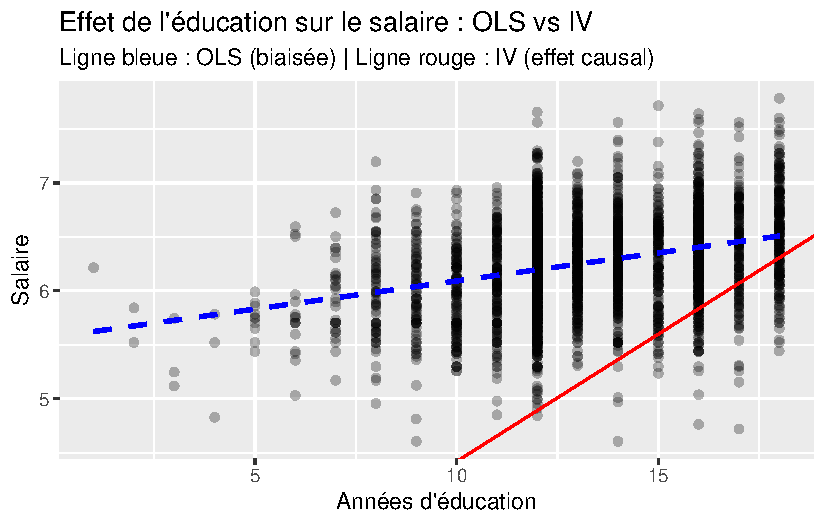
\includegraphics[keepaspectratio]{projet_VI_files/figure-pdf/unnamed-chunk-15-1.pdf}}

\section{Interpretation}\label{interpretation}

Avec la regression (mco), Une année d'éducation augmente le salaire de
7,9\% Avec la correction de l'endogénéité par la variable instrumentale,
Une année d'éducation augmente le salaire de 23.6\%

\#Diagnostique

\begin{Shaded}
\begin{Highlighting}[]
\FunctionTok{summary}\NormalTok{(model\_2sls)}
\end{Highlighting}
\end{Shaded}

\begin{verbatim}

Call:
iv_robust(formula = salaire ~ education + sud + exper_marche + 
    experience + race_noir | proximite + sud + race_noir + exper_marche + 
    experience, data = base, diagnostics = TRUE)

Standard error type:  HC2 

Coefficients:
              Estimate Std. Error t value  Pr(>|t|)  CI Lower CI Upper   DF
(Intercept)   2.059314  0.7692794   2.677 7.470e-03  0.550947  3.56768 3004
education     0.235982  0.0445478   5.297 1.260e-07  0.148634  0.32333 3004
sud          -0.044578  0.0299769  -1.487 1.371e-01 -0.103355  0.01420 3004
exper_marche -0.002458  0.0004479  -5.488 4.398e-08 -0.003336 -0.00158 3004
experience    0.150583  0.0201193   7.484 9.382e-14  0.111134  0.19003 3004
race_noir    -0.032562  0.0456081  -0.714 4.753e-01 -0.121989  0.05686 3004

Multiple R-squared:  -0.2252 ,  Adjusted R-squared:  -0.2273 
F-statistic: 74.35 on 5 and 3004 DF,  p-value: < 2.2e-16

Diagnostics:
                 numdf dendf value  p.value    
Weak instruments     1  3004 32.93 1.05e-08 ***
Wu-Hausman           1  3003 21.02 4.73e-06 ***
Overidentifying      0    NA    NA       NA    
---
Signif. codes:  0 '***' 0.001 '**' 0.01 '*' 0.05 '.' 0.1 ' ' 1
\end{verbatim}

\begin{itemize}
\item
  Test des instruments faibles: L'instrument est fort car F-Stat
  \textgreater{} 10 (32,93)
\item
  Test de Hausman (endogénéité) On rejette H0 d'exogénéité de la
  variable education. (p-value : 4.73e-06)
\end{itemize}

*Test de sur-identification

Ce test n'a pas été éffectué car le modèle est juste identifié (nombre
de variable explicative = nombre de variables instrumentales)

En resumé :

Nous avons utilisé la proximité d'une université comme instrument pour
corriger l'endogénéité du niveau d'éducation dans l'explication du
salaire. Le test de Hausman confirme l'endogénéité, justifiant le modèle
IV. Les tests indiquent que l'instrument est valide (fort), et nous
observons qu'une année supplémentaire d'éducation augmente le salaire
d'environ 23,6 \%, toutes choses égales~par~ailleurs.




\end{document}
